\chapter{Electrodomésticos}
A continuación presentaré los principales componentes que se encuentran en los aparatos eléctricos y electrodomésticos.

\section{Los interruptores}
{\large \textbf{a) Interruptores, inversores y pulsadores}}\\

\noindent\begin{minipage}[t]{0.35\textwidth}\vspace{0pt}

El interruptor más básico es un sistema para cerrar y abrir un
circuito eléctrico, ya sea a tensión de red u otra señal eléctrica.
Su límite será la corriente que puede pasar a través de ellos sin
dañarlos.\\

\begin{flushleft}
Hay interruptores dobles que permiten abrir y cerrar dos circuitos
en paralelo y una variante conocida como conmutador que permite conectar un pin común a
cualquiera de sus otras dos patillas. Existen más complejos: triple,
cuádruple, etc. Pero el principio sigue siendo el mismo
\end{flushleft}
\end{minipage}% Don't leave empty lines and empty chars between minipages
\hfill%
\begin{minipage}[t]{0.6\textwidth}\vspace{0pt}
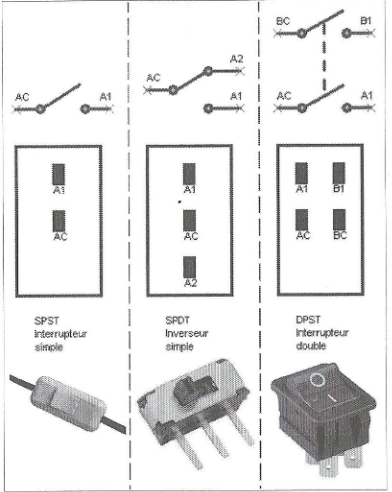
\includegraphics[width=\linewidth]{tipos-interruptores}
\end{minipage}
\vspace{1em}

Se comprueban simplemente con el multímetro en modo continuidad y aislamiento
(véase el capítulo 2.4.b).
\newpage

Otro tipo de interruptor que se encuentra generalmente soldado en placas electrónicas es el "botón pulsador", su particularidad es que sólo cierra el circuito mientras está pulsado, y lo abre al soltarse.
Existen de 2 y de 4 patillas, como en la foto, sin embargo las patillas están conectadas internamente 2 a 2 de cada lado y sólo es capaz de conmutar 1 circuito.

\begin{figure}[h]
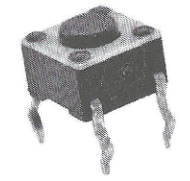
\includegraphics[width=0.25\linewidth]{boton-pulsador}
\centering
\end{figure}

Se encuentran encontrará detrás de cada botón de un equipo de alta fidelidad, reproductor de CD/DVD, ordenador portátil (aparte del teclado), pantalla, etc,
El popular modelo de arriba hace un pequeño "clic" al pulsarlo.\\

\textbf{Fallos comunes:}
\begin{itemize}
\item Mal contacto eléctrico interno, que provoca una alimentación intermitente o chispazos (en pulsadores no):
\\

$\blacktriangleright$ Si puedes desmontar la pieza (es el caso sobre todo de los interruptores como el anterior), intenta comprender qué partes que partes necesitan hacer contacto. En los interruptores que controlan la tensión de red, suele ocurrir que en el punto preciso
donde se hace el contacto, el metal está ennegrecido e impide un buen contacto eléctrico.
En este caso, a menudo basta con limpiar con una pequeña lima o papel de lija para restablecer un buen contacto eléctrico, seguido de una limpieza con alcohol de 90° o spray "limpia contacto".
\\

En el caso de los interruptores pequeños o pulsadores que no se pueden desmontar, echar limpiacontactos puede ser suficiente para darles una nueva vida. Si no, han de ser reemplazados, suelen ser muy baratos.

\item Ausencia de contacto
\\

$\blacktriangleright$ Si puede desmontarse, comprueba que no se ha movido ninguna pieza del interior.
A menudo habrá que sustituir toda la pieza.
\\
\end{itemize}
\newpage

\textbf{b) Un interruptor particular: el temporizador}

\noindent\begin{minipage}[t]{0.5\textwidth}\vspace{0pt}
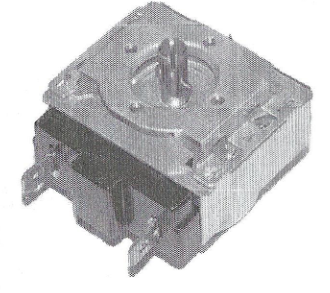
\includegraphics[width=\linewidth]{temporizador}
\end{minipage}
\hfill%
\begin{minipage}[t]{0.4\textwidth}\vspace{\fill}
\vspace{\fill} % Add this to push the text down
Es un interruptor, excepto que se utiliza para cerrar el circuito,
que se abrirá de nuevo cuando haya transcurrido el tiempo deseado.
Se prueba como un interruptor simple.
\vspace{\fill} % Add this to push the text down
\end{minipage}
\vspace{1em}

\section{Sensores}

Un sensor es un elemento que recibe y transmite una información: posición de un elemento (por diferentes métodos: mecánica, óptica, magnética...), movimiento, temperatura, presión...

Transmite esta información de forma eléctrica (interruptor abierto/cerrado, resistencia variable).

Algunos sirven directamente para cotar la alimentación eléctrica.
Otros, como el sensor de efecto hall, requieren otros componentes electrónicos para ser interpretados.\\

\begin{center}
\textbf{a) Sensores de posición mecánica}
\end{center}
\begin{minipage}[h]{\textwidth}\vspace{0pt}
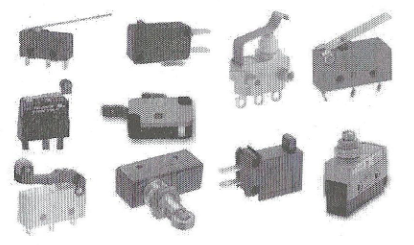
\includegraphics[width=0.6\linewidth]{sensores-posicion-mecanica}
\centering
\end{minipage}

Se encuentran en muchos aparatos, pueden servir para verificar si una puerta está bien cerrada (horno microondas) o la presencia de una tapa/recipiente (batidora, blender)
\newpage

A menudo están cableados en serie (véase cap. 2.4.4) con la alimentación del elemento potencialmente peligroso (motor que hace girar las cuchillas, etc.).
Es una fuente de averías muy frecuente. Suele tener 2 ó 3 clavijas:

\begin{itemize}
\item 2 patillas, es un interruptor clásico, verifica que esté en modo abierto (sin continuidad) en la posición "OFF" y en posición cerrada (con continuidad) en la posición "ON".
\item 3 patillas, es un conmutador. Tiene 3 patillas llamadas Reposo, Trabajo y Común.
\end{itemize}


\noindent\begin{minipage}[t]{0.35\textwidth}\vspace{0pt}
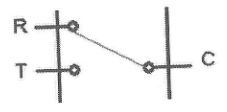
\includegraphics[width=\linewidth]{conmutador}
\end{minipage}
\hfill%
\begin{minipage}[t]{0.6\textwidth}\vspace{\fill}
\vspace{\fill} % Add this to push the text down
Cuando está en posición de reposo (obligado por un muelle, cuando no hay presión): Hay contacto entre la patilla C y R, y no hay contacto entre la T y las 2 otras.\\
\vspace{\fill} % Add this to push the text down
\end{minipage}
\vspace{1em}

Cuando está en posición de trabajo, C y T están en contacto y no hay contacto entre R y las otras 2.

A menudo hay que deducir a qué corresponde cada patilla, ya que no siempre están etiquetadas. Verifica bien que no haya ningún cortocircuito indeseado, ni ningún circuito abierto indeseado según la posición, y que los estados conmutan al accionar el conmutador.

\begin{center}
\textbf{b) Sensores de temperatura}
\end{center}

\begin{itemize}

\item El termostato mecánico regulable

\noindent\begin{minipage}[t]{0.45\textwidth}\vspace{0pt}
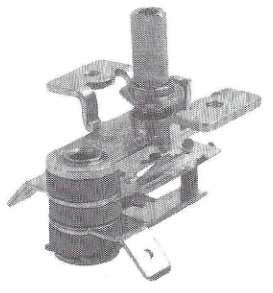
\includegraphics[width=\linewidth]{termostato}
\end{minipage}
\hfill%
\begin{minipage}[t]{0.5\textwidth}\vspace{\fill}
\vspace{\fill}
No es ni más ni menos que un interruptor
que se abre y se cierra en función de la
temperatura deseada.

Se trata de una función muy común en
electrodomésticos: hornos, planchas, calentadores eléctricos
plancha, calentador eléctrico, placa
hornillos, etc.

Se comprueba del mismo modo que un interruptor.
Oirá un pequeño "clic" cuando se enciende el termostato. Este chasquido suele significar que está funcionando correctamente.\\
\vspace{\fill}
\end{minipage}
\vspace{1em}
\\

\item El klixon

\begin{normalize}
\begin{minipage}[h]{\textwidth}\vspace{0pt}
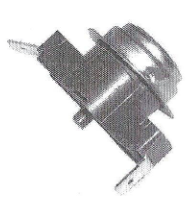
\includegraphics[width=0.3\linewidth]{klixon}
\centering
\end{minipage}

Se trata de un seguro térmico. 
Se encuentra por ejemplo en lavadoras, en el interior de la cuba.
Cuando la temperatura sobrepasa cierto límite, se abre y corta la corriente.
Cuando es rearmable, suele tener un botón que permite volver a conectarlo (hasta la próxima vez que se exceda la temperatura)

Cuando ocurre un sobrecalentamiento suele ser por un fallo del termostato, que no ha regulado bien la temperatura del aparato y ha provocado un sobrecalentamiento.
El klixon se testea con el modo continuidad.
\end{normalize}

\item La sonda térmica

\begin{normalize}
\begin{minipage}[h]{\textwidth}\vspace{0pt}
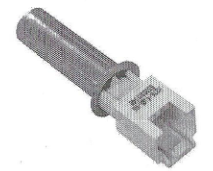
\includegraphics[width=0.3\linewidth]{sonda-termica}
\centering
\end{minipage}

Es una resistencia variable por temperatura, según el modelo, su resistencia aumentará o disminuirá con la temperatura.
Se encuentran en diferentes formas en una gran variedad de electrodomésticos.
El modelo de la foto se encuentra en algunas lavadoras.
\\

Está conectado principalmente a una tarjeta electrónica que controla la
temperatura.

En general, si se obtiene un valor de resistencia que no sea ni cortocircuito ni infinito, hay muchas posibilidades de que el sensor esté en buen estado.
En el caso de sensores en contacto con el agua, como éste, la cal adherida al sensor 
puede ser responsable de un problema de regulación de la temperatura.
En este caso, basta con limpiarlo con vinagre blanco.
\end{normalize}

\end{itemize}
\newpage
\begin{center}
\textbf{c) Sensores de posición por campo magnético}
\end{center}
Se encuentran a menudo en electrodomésticos, para detectar la presencia de agua en un depósito (cafetera, plancha, ...) o captar la posición del tambor en una lavadora.\\


Hay dos grandes familias:

\begin{itemize}
\item Los sensores "ILS", que funcionan como un interruptor abierto o cerrado según la presencia de un imán a proximidad.

\begin{figure}[h]
\centering
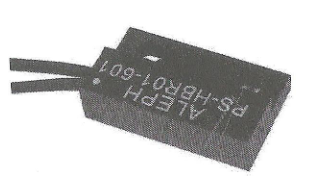
\includegraphics[width=0.6\linewidth]{sensor-ILS}
\caption*{\textit{Tipo "ILS": Sensor de posición del tambor de una lavadora}}
\end{figure}

\item Los sensores de "efecto hall", que hacen variar la tensión de sus contactos según la intensidad del campo magnético a proximidad.

\begin{figure}[h]
\centering
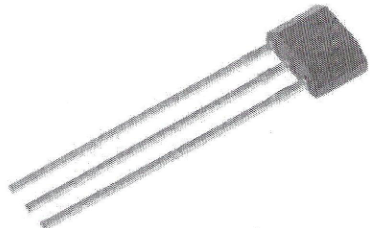
\includegraphics[width=0.6\linewidth]{sensor-hall}
\caption*{\textit{Tipo "efecto hall"}}
\end{figure}

\end{itemize}
\newpage 

\begin{center}
\textbf{d) Sensores de presión (presostatos)}
\end{center}
Se pueden encontrar en lavadoras, generadores de vapor, lavadoras, máquinas expreso.... Constan de 1, 2 o incluso 3 conmutadores "común - reposo/trabajo" que conmutan en función de la presión que reciben.

\noindent\begin{minipage}[t]{0.4\textwidth}\vspace{0pt}
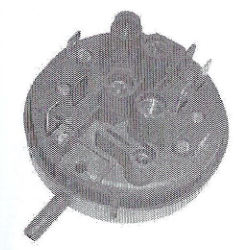
\includegraphics[width=\linewidth]{sensor-presion}
Presostato de una lavadora
\end{minipage}
\hfill%
\begin{minipage}[t]{0.5\textwidth}\vspace{\fill}
\vspace{\fill}
En el caso de los presostatos de las
lavadoras, la presión es una imagen del nivel de
nivel de agua en la máquina.
Los nombres de las clavijas suelen ser
así:
\\

Dígito de las decenas: nivel de agua (1 para
$1^{er}$ nivel...)
Dígito de las unidades: 1: común / 2 :
resto / 3: trabajo\\
\vspace{\fill}
\end{minipage}
\vspace{1em}

\begin{figure}[h]
\centering
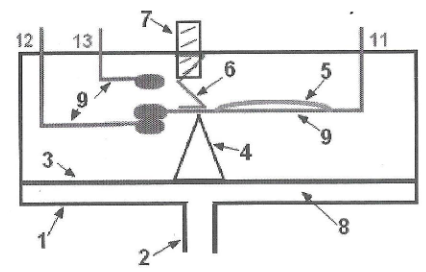
\includegraphics[width=0.6\linewidth]{esquema-presostato}
\caption*{\textit{Esquema de un presostato}}
\end{figure}

\textbf{Funcionamiento:\\}
En reposo, el muelle "6" hace contacto entre "11" y "12".
el aire comprimido por el agua del depósito llega a "2", presiona sobre la membrana "3" y después sobre la aguja "4".
El efecto de esta presión es forzar a la lengüeta "9", conectada a "11", a 
desconectarse de "12" y conectarse a "13".

\newpage
\section{Resistencias calefactoras}

Todos los conductores emiten calor cuando la corriente fluye por ellos, pero cuando hablamos de resistencia calefactora, hablamos de un "hilo" conductor que ha sido diseñado específicamente para tener una cierta resistencia eléctrica, y que es capaz de aguantar una temperatura muy alta.
Estos tipos de artilugios se encuentran en todos los aparatos que necesitan producir calor: hornos eléctricos, tostadoras, hervidoras de agua, planchas, gofreras, freídoras eléctricas, lavadoras, lavavajillas...
En general se alimentan de la corriente alterna 220V. Cuando no están en el interior de una carcasa indesmontable, tienen esta apariencia:

\begin{figure}[h]
\noindent\begin{minipage}[t]{0.26\textwidth}\vspace{0pt}\
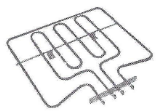
\includegraphics[width=\linewidth]{resistencia-horno}
Resistencia de un horno
\end{minipage}
\begin{minipage}[t]{0.26\textwidth}\vspace{0pt}
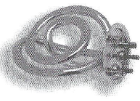
\includegraphics[width=\linewidth]{resistencia-hervidora-de-agua}
Resistencia de una hervidora de agua
\end{minipage}
\begin{minipage}[t]{0.26\textwidth}\vspace{\fill}
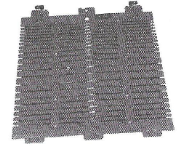
\includegraphics[width=\linewidth]{resistencia-tostadora}
Resistencia de una tostadora
\end{minipage}
\centering
\end{figure}
\vspace{1em}

Para comprobar el buen estado de una resistencia, remitirse al capítulo 2.4b. El valor de una resistencia calefactora generalmente es alrededor de 10 $\Omega$\\

\noindent\fbox{%
    \parbox{\textwidth}{%
Una resistencia de 50 $\Omega$ sometida a una tensión de 230V proveerá una potencia de alrededor 1000W $(P=U^2/R)$
    }%
}\\

Para encontrar los contactos de una resistencia, basta con seguir el hilo calefactor, o el tubo que lo envuelve, a veces hay varios en paralelo, como en los hornos.
También hay que verificar el aislamiento de la resistencia para aquellas que están envueltas en un tubo metálico (horno, lavadora, hervidora...).
Para ello, pon el multímetro en el valor $\Omega$ más alto (no en modo continuidad) y coloca una punta en una extremidad de la resistencia, y la otra en el tubo metálico: deberías obtener una resistencia infinita.
Si no es el caso, la carcasa metálica del aparato estará conectada a un potencial eléctrico, y sería conveniente reemplazar la resistencia, incluso aunque no haga saltar el diferencial, ya que existe un riesgo potencial.
\newpage
\section{Las bombas}
Su función es hacer circular un líquido.
Antes de culpar a la bomba, es conveniente verificar que los tubos y conectores situados antes/después de la bomba no estén taponados o agujereados. En general, se alimentan directamente de la red. Encontramos 2 tipos de bombas, que no tienen la misma forma ni función.\\


\begin{large}
\textbf{a) Bomba rotativa (o radial)}
\end{large}

\noindent\begin{minipage}[t]{0.3\textwidth}\vspace{0pt}
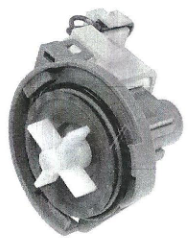
\includegraphics[width=\linewidth]{bomba-rotativa}
\end{minipage}
\hfill%
\begin{minipage}[t]{0.6\textwidth}\vspace{\fill}
\vspace{\fill}
\begin{flushleft}
Consiste en un motor que hace girar una hélice, no permite que la presión sea muy alta.\\


Se encuentra principalmente en lavadoras y lavavajillas, tiene como función vaciar la máquina de agua. Se encuentra justo antes del tubo de desagüe acanalado.
\end{flushleft}
\vspace{\fill}
\end{minipage}
\vspace{1em}

Para probarlas, la mejor manera es desconectar los 2 contactos (3 si hay tierra), y conectarla directamente a la red eléctrica (ver capítulo 3.1.a). Si no gira, está fuera de servicio. A veces gira muy lentamente, lo que le impide cumplir su función, en estos casos suele bibrar y hacer un ruído anormal.\\


\begin{large}
\textbf{a) Bomba "ULKA" (o bomba de vibración u oscilante)}
\end{large}

\noindent\begin{minipage}[t]{0.5\textwidth}\vspace{0pt}
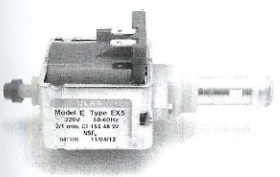
\includegraphics[width=\linewidth]{bomba-ulka}
\end{minipage}
\hfill%
\begin{minipage}[t]{0.5\textwidth}\vspace{\fill}
\vspace{\fill}
\begin{flushleft}
Está constituída por un piston que vibra en su interios, gracias a un campo magnético producido por una bobina por la que pasa corriente. Es capaz de producir mucha más presión que la mayor parte de bombas rotativas, y por esta razón se suele utilizar en máquinas expresso y centros de vapor.
\end{flushleft}
\vspace{\fill}
\end{minipage}
\vspace{1em}

Para probarlas, conecta los 2 terminales a la red eléctrica (evitar aguantarla con la mano, en caso tuviese un fallo de aislamiento), si vibra, generalmente funciona.

\newpage
\section{Las electroválvulas}

\noindent\begin{minipage}[t]{0.4\textwidth}\vspace{0pt}
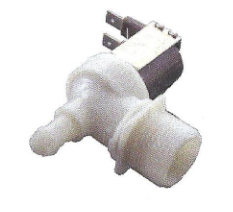
\includegraphics[width=\linewidth]{electrovalvula}
\end{minipage}
\hfill%
\begin{minipage}[t]{0.5\textwidth}\vspace{\fill}
\vspace{\fill}
\begin{flushleft}
Su función es bloquear o permitir el paso de un líquido a presión, están formados por una bobina que crea un campo magnético
para abrir el paso a través de una pieza metálica
que se desliza.\\

Se utilizan principalmente en lavadoras y lavavajillas para dejar pasar el agua, se sitúan justo después de la tubería de entrada de agua.

\end{flushleft}
\vspace{\fill}
\end{minipage}
\vspace{1em}

\begin{figure}[h]
\centering
\textbf{Esquema de una electroválvula}
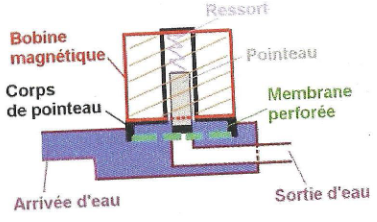
\includegraphics[width=0.65\textwidth]{esquema-electrovalvula}
\end{figure}

Puede tener dos fallos:
\begin{itemize}
\item Siempre deja pasar el agua, en este caso la máquina se llena contínuamente mientras no se corte la llegada de agua, se suele tratar de una junta agujereada, que a veces se puede cambiar.
\item Nunca deja pasar el agua, en este caso, une los dos contactos a la red (sin tocarla con la mano, en caso hubiese fallo de aislamiento), si vibra, en general es que funciona, si el agua está conectada debería dejar pasar el agua. Si no hace ningún ruído ni deja pasar el agua, probablemente el bobinado esté dañado (A veces también se puede acumular cal en el mecanismo, en cuyo caso se puede limpiar con vinagre blanco).
\end{itemize}
\newpage

\section{Los motores}

Un motor se compone de dos partes principales: el stator (o inductor), que está fijo, y el "rotor" (o inducido), que es la parte que gira. Hay distintos tipos de motores (de corriente contínua, universal, paso a paso...) pero abordaré el motor más utilizado en el mundo de la electrodoméstica: el motor universal (o serie).
"Universal" porque puede funcionar con corriente alterna o contínua. "Serie" porque los bobinados del stator y el rotor están cableados en serie. Se encuentra en lavadoras, herramientas de mano, aspiradoras, batidoras...
Se reconoze por los dos embobinados grandes del stator, de láminas de cobre, y por sus escobillas:
\begin{figure}[h]
\centering
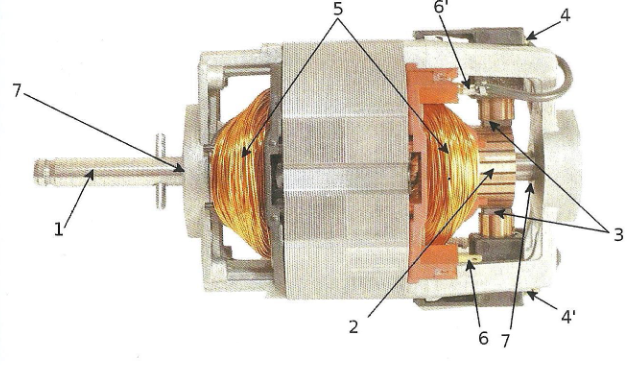
\includegraphics[width=\textwidth]{motor-universal}
\end{figure}


\begin{tabularx}{\textwidth}{|X|X|}
\hline
\begin{enumerate}
	\setlength\itemsep{0em}
    \item Eje de rotación
    \item Laminas de cobre o colectores
\end{enumerate}
&
\begin{enumerate}
	\setlength\itemsep{0em}
	\setcounter{enumi}{2} % Set the counter to continue numbering
    \item Escobillas o carboncillos
    \item Conectores de las escobillas
    \item Bobinas de stator
    \item Conectores de las bobinas del stator
    \item Rodamientos
\end{enumerate} \\
\hline
\end{tabularx}

\noindent\fbox{%
    \parbox{\textwidth}{%
\textbf{Principio de funcionamiento:}\\
La corriente entra por el conector (6) y atraviesa el primer bobinado del stator (5) $\rightarrow$ (6') $\rightarrow$ (4) $\rightarrow$ la escobilla superior (3) $\rightarrow$ la lámina de contacto con la escobilla superior (2) $\rightarrow$ una bobina del rotor $\rightarrow$ la lámina de contacto opuesta a la primera $\rightarrow$ la escobilla de abajo (3) $\rightarrow$ (4') $\rightarrow$ el segundo embobinado del stator y vuelve a salir por el segundo conector, idéntico a (6)\\

El paso de la corriente por las bobinas del stator tiene el efecto de generar un campo magnético cuya dirección sería la línea que parte de tus ojos, atravesando el motor por el centro, en medio de las bobinas del stator. La bobina del rotor, recorrida por la misma corriente, crea igualmente un campo magnético que se alinea con el primero, lo que hace girar el motor unos grados. Al girar, se alinean otras láminas colectores)y alimentan otra bobina del rotor, que a su vez de alineará con el campo magnético del stator, y así sucesivamente, haciendo girar al motor.
    }%
}\\

\textbf{a) Síntomas y diagnósticos}
\begin{enumerate}
\item El motor emite un zumbido, pero no gira, gira muy lentamente o con dificultad
\end{enumerate}

{\small \textbf{a) problema mecánico}\\}

Desenchufa siempre el aparato antes.
Intenta girar el motor con la mano. Si resulta imposible o difícil asegúrate de que el motor sólo acciona su propio eje retirando un engranaje o una correa, por ejemplo, o sacando el motor de su motor de su ubicación.
Si el eje del motor gira libremente con la mano, significa que el problema
proviene de la pieza accionada por el eje y debe bloquearse.
Si el eje sigue siendo difícil de girar, pruebe a poner un poco de aceite en los cojinetes en los rodamientos de ambos lados.
Si el eje está completamente bloqueado, utiliza un poco de desengrasante tipo WD40,
déjelo actuar unos minutos y vuelva a intentarlo.
Si el resultado no es satisfactorio, pruebe a desmontar el rotor (si es posible) para limpiarlo y engrasarlo a fondo.
Tenga cuidado de retirar las escobillas de carbón antes del desmontaje para evitar romperlas durante el reensamblaje. Si todo parece mecánicamente normal, pase al siguiente paso.

